\documentclass[a4paper,11pt,twocolumn]{article}
\usepackage{verbatim}
\usepackage[dvipdf]{graphicx}

% \newcommand{\intro}[1]{\emph{#1}}


\begin{comment}
\textwidth = 6.5 in
\textheight = 9 in
\oddsidemargin = 0.0 in
\evensidemargin = 0.0 in
\topmargin = 0.0 in
\headheight = 0.0 in
\headsep = 0.0 in
\parskip = 0.2in
\parindent = 0.0in
\end{comment}

\author{Rafael A. Calvo \and Ken Williams}
\title{ASX Corporate Announcements Categorization}
\begin{document}

\maketitle

\begin{center}
School of Electrical and Information Engineering\\
The University of Sydney\\
Bldg J03, Sydney NSW 2006\\
\{rafa, kenw\}@ee.usyd.edu.au

\end{center}

\section{Abstract}

This paper compares the performance of several machine learning algorithms with results for the automatic categorization of corporate announcements in the Australian Stock Exchange (ASX)  Signal G data stream. The article also describes some of the numerous applications that the categorization of corporate announcements may enable. We have performed tests on two categorization tasks: market sensitivity, which indicates whether an announcement will have an impact on the value of some stocks, and report type, which classifies the announcements into one of the report categories defined by the ASX. We have tried Neural Networks, Na�ve Bayes classifiers, and Support Vector Machines and achieved high precision and recall.

\section{Introduction}

The Australian Stock Exchange Limited (ASX - http://www.asx.com.au/) operates Australia�s primary national stock exchange.  Companies listed on ASX are required under the Listing Rules to make announcements about their activities "in order to ensure a fully informed market is maintained."   In order to guarantee access to this information, stock exchanges such as the ASX publish all recent and historical company announcements.  Thanks to language technologies such as automatic document categorization, these corporate announcements can provide new sources of valuable financial information. 

We have used the Signal G corpus, an electronic signal from the ASX that provides subscribers with details of company announcements issued by the relevant company or the ASX in accordance with listing rules.

Under the ASX Company Announcement Platform (CAP), company announcements are lodged by fax or hand delivery to a centralised company announcements office where they are put into electronic format and delivered to users of the signal. The announcements are delivered in full text or summarized (depending on the length). 
Signal G is available to the public, member organizations and information vendors. 

In this paper we assess the performance of several machine learning classifiers on this corpora, namely Neural Networks, Na�ve Bayes, and Support Vector Machines on two tasks: ``report type'' and ``market sensitivity'' categorization. Report-type is ``a code to categorize company announcements'' that indicates categories such as ``annual report'' or ``takeover announcement.'' Signal G has 144 report types with a very skewed distribution: some report types have many documents, some have very few.

The second task, market sensitivity, indicates whether the associated company announcement contains information that may influence trading in the issuing company. This allows users of this data to select which announcements are critical. 

The next section of this paper will discuss the problem and application domain area, emphasizing the importance of language technologies in the financial information arena. The third section discusses the data set used. Section four describes the different machine learning techniques and the application framework that we have implemented in order to perform these types of categorization tasks. The fourth section describes the quantitative results and section five concludes.



\section{Problem Setting}

Corporate announcements have provided valuable information to traders and the general public for decades. For this reason these announcements are used by regulators as the main tool to keep the market informed of all important events. The law assumes that these public announcements contain all the information needed by an individual trader to keep a reasonable understanding of what is happening with a particular company. This allows investors to make decisions based on information that is up to date and is equivalent to the information that company insiders might have. There is little doubt about the value of the information contained in these announcements, and there are a number of research groups developing novel applications using this data. These applications include alert systems where brokers receive notification (e.g. over email or SMS) of important announcements, intelligent repositories where the information shown to users is filtered using ``information profiles'' that they can build, and several other applications that require the automatic processing of announcements.  We describe in this article the evaluation of categorization techniques used to build these applications.

A categorizer will assign a category in one of the above two sets (sensitivity or report type) to each document in the test set. Since documents in the test set have not been used to adjust the parameters of the classifier it is normally assumed that the performance on new data would be similar. 

Machine learning algorithms such as Neural Networks can iteratively learn non-linear mappings from a set of training patterns, while others such as Decision Trees and Na�ve Bayes classifiers build these mappings by computing class probabilities or feature-class entropy scores. 


\section{Data Description}

The corpus was built from the Signal G announcement stream from the Australian Stock Exchange (ASX).

The ASX Data Services is a financial information service providing daily market information from the Stock Exchange Automated Trading System (SEATS), ASX futures and the company announcement service. All daily stock exchange activity is available in different electronic data feeds that the ASX calls ``signals''. Signal G is an electronic signal that provides subscribers with details of companies� announcements. The ASX�s Company Announcement Platform (CAP) receives the announcements produced by organizations (by fax, email or other means), processing and centralizing all the information that is then delivered through the Signal G feed. The processing includes several procedures such as summarization (if the announcement is too long) and a manual categorization to a set of predefined categories. After this categorization process each announcement (document) is assigned to one of 144 report types, or can also be classified as market sensitive or not. From the total 136,630 documents used, 46,530 are marked as sensitive and 90,100 as not sensitive. For this last assignment the human classifier (based on experience) states whether or not the document may have an effect on the value of the share, volume of trading, or other market measurements.



\begin{table}
\begin{tabular}{|r|r|r|r|}
\hline
 & Sensitive & Nonsensitive & Totals \\
\hline
Training & 32458 & 63067 & 95525 \\
\hline
Test & 14072 & 27033 & 41405 \\
\hline
Totals & 46530 & 90100 & 136630\\
\hline
\end{tabular}
\caption{Signal G corpus (number of documents)}
\label{signalg}
\end{table}

In order to build a corpus that could easily be used by other researchers, the Signal G data was first parsed into XML. In this parsing we extracted semantic fields not included in the original Signal G data. So far, these include the name of the signing person and their role (e.g. Managing Director).

Each document was assigned a document ID, one or more classes that it belongs to (related industry or type of news), a title and the main text. 


\section{Methods}

We have compared four machine learning methods that have provided some of the best performances in other classification tasks (Yang and Liu 1999). Support Vector Machines (SVM), Na�ve Bayes (NB), and Neural Networks (NN) encompass a wide set of algorithms. It is not possible to describe them thoroughly in this article, so we will only summarize those issues that might be required to reproduce the results.

The algorithms (except for NN) have been implemented within the AI::Cat\-e\-go\-riz\-er framework, an open source categorization framework written in Perl. The framework has been designed to facilitate the construction of new categorization applications following industry best practices (Fayad and Schmidt 1999).

Support Vector Machines were developed by Vapnik and colleagues during 1995-1996 (Cortes \& Vapnik 1995, Sch�l\-kopf et. al. 1999). They were first used in document categorization by Joachims (1998, 1999) and used by other authors in experimental comparisons with other methods (Yang \& Liu, 1999).

Naive Bayes are one of the several well-studied probabilistic classifiers (Lewis, 1998). Most document classification research using probabilistic methods uses NB, so a number of authors have described them and shown experimental results on a number of data sets (Joachim 1998, Yang ...). 

Neural Networks have been widely used and described in the document classification literature (Yang \& Liu 1999, Calvo \& Ceccatto 2000, Calvo 20001). The neural network parameters are adjusted to the training data in a number of iterations. We have used a backpropagation algorithm that minimizes quadratic error. The input layer has as many units (neurons) as document features retained. The number of hidden units is determined by optimising the performance on a cross-validation set. There is one output unit for each possible class, with activation values between 0 and 1. If one (or more) of the output units has activation greater than 0.5, the classifier will state that the document belongs to that (those) categories. 


\section{Results}

Table \ref{contingency} describes the possible outcomes of a binary classifier.  The ``assigned'' YES/NO results refer to the classifier output and the ``correct'' YES/NO refers to the manual ASX-assigned categories. The perfect classifier would have a value of 1 for $a_j$ and $d_j$, and 0 for $b_j$ and $c_j$.

\begin{table}
\begin{tabular}{|r|r|r|}
\hline
& \multicolumn{2}{|c|}{Correct} \\
\hline
Assigned & YES & NO \\
\hline
YES & $a_j$ & $b_j$ \\
\hline
NO & $c_j$ & $d_j$ \\
\hline
\end{tabular}
\caption{Contingency table for class $j$}
\label{contingency}
\end{table}

Using Table \ref{contingency} we define three performance measures common in the document categorization literature. 

\begin{displaymath}
recall = r = \frac{a}{a+c} \quad \textrm{if} \enspace a+c>0, 0 \enspace \textrm{otherwise}
\end{displaymath}

\begin{displaymath}
precision = p = \frac{a}{a+b} \quad \textrm{if} \enspace a+b>0, 0 \enspace \textrm{otherwise}
\end{displaymath}

These two measures contain information about whether classification errors are dominated by false positives or false negatives.  The trade-off between recall and precision can often be controlled by setting a classifier�s parameters. Both measures should typically be used to describe the overall performance, as neither is particularly informative by itself. Another common performance measure is the $F_\beta$ measure:

\begin{displaymath}
F_\beta = \frac{(\beta^2 + 1)pr}{\beta^2 p + r}
\end{displaymath}

The most commonly used $F_\beta$ measure in document categorization is $F_1$, which evenly balances precision and recall:

\begin{displaymath}
F_1 = \frac{2pr}{p + r}
\end{displaymath}

When dealing with multiple classes there are two possible ways of averaging these measures, \emph{macro-averaging} and \emph{micro-averaging}. In macro-averaging, one contingency table per class is used, then performance measures are computed on each of them and averaged. In micro-averaging only one contingency table is used; an average of all the classes is computed for each cell and the performance measures are obtained therein. The macro-average weights equally all the classes, regardless of how many documents they contain. The micro-average weights equally all the documents, thus biasing toward the performance on common classes.

Different classifiers will perform differently on common and rare categories. Learning algorithms are trained more often on more populated classes thus risking local overfitting.

We summarize here the general steps followed in the preparation of the experiments, and the results therein. 

\begin{table}
\begin{tabular}{|l|l|l|l|l|l|}
\hline
& Stopwords & Stemming & Feature Reduction & TF/IDF & Architecture\\
\hline
NN & ??? & Yes & $\chi^2$ & LTC? (Need to find out what this really was) & 1000 inputs, 50 hidden units. \\
\hline
NB & SMART & Yes & DF & TXX & 1000 features \\
\hline
SVM & SMART & Yes & DF & TXX & 1000 features, linear kernel \\
\hline
\end{tabular}
\caption{Comparative description of algorithms used}
\label{algos}
\end{table}

\begin{enumerate}

\item Linguistic dimensionality reduction: A list of stopwords (Salton 1989) was removed from the document collection and the Porter stemming algorithm was applied (Manning and Sch�tze 1999).
\item Statistical dimensionality reduction: Chi squared, document frequency, and other statistics are often used to reduce the feature vector dimensionality (Manning and Sch�tze 1999; Sebastiani 2002).
\item Vectorization and weighting: The resulting documents were represented as vectors, using TF/IDF weighting (Salton and Buckley 1988; Yang and Pedersen 1997). 
\item Architecture: The selected terms were used as input features to the classifier. Some of the algorithms allow several architectures, and the best algorithm was chosen by optimising the results on a cross-validation set. 
\item Training: We generated a cross-validation set randomly. These documents were set aside and the Neural Network was trained on the remaining ones. 

\end{enumerate}

\begin{table}
\begin{tabular}{|c|c|c|c|c|c|c|}
\hline
   & \multicolumn{3}{|c|}{Micro} & \multicolumn{3}{|c|}{Macro} \\
\hline
   & $p$  & $r$  &$F_1$ & $p$  & $r$  & $F_1$ \\
\hline
 NN & 0.89 & 0.89 & 0.89 & 0.88 & 0.88 & 0.88 \\
 NB & 0.83 & 0.84 & 0.83 & 0.90 & 0.90 & 0.90 \\
SVM & 0.82 & 0.82 & 0.82 & 0.80 & 0.79 & 0.80 \\
\hline
\end{tabular}
\caption{Performance for the market sensitivity task}
\label{res:sens}
\end{table}


\begin{table}
\begin{tabular}{|c|c|c|c|c|c|c|}
\hline
   & \multicolumn{3}{|c|}{Micro} & \multicolumn{3}{|c|}{Macro} \\
\hline
   & $p$  & $r$  &$F_1$ & $p$  & $r$  & $F_1$ \\
\hline
NN & 0.87 & 0.71 & 0.78 & 0.45 & 0.34 & 0.37  \\
NB & 0.62 & 0.67 & 0.64 & 0.46 & 0.61 & 0.46  \\
SVM &  &  &  &  &  & \\
\hline
\end{tabular}
\caption{Performance for the report type task}
\label{res:rept}
\end{table}

It is important to note that the performance results are based on comparing the automatic categorization of each document with the tagging of human experts at the ASX. The manual classification is a subjective decision process affected by the ASX�s legal liabilities and the normal human classification disagreements. It has been shown in various studies that there could be considerable variation in the inter-indexer agreement (Bruce and Wiebe 1998; Brants 2000). For example, in a Reuters news collection correction rates averaged 5.16\% (Rose, Stevenson et al. 2002) with some editors being corrected up to 77\% of the time. Similar disagreements can be expected in the ASX�s assignments on the Signal G corpus.  In the light of these disagreements we can imagine that there might be a limit to the performance that can be obtained by automatic categorization. 

Figure \ref{histogram} shows a histogram of classes and documents for different performance ranges using the Na�ve Bayes classifier. It shows how most categories that do well have large number of documents, except for some that have very few documents (fewer than 5). This shows the well-known result that the machine learning algorithms such as Na�ve Bayes perform better on well-populated categories. Similar results can be obtained for the other classifiers.

\begin{figure}
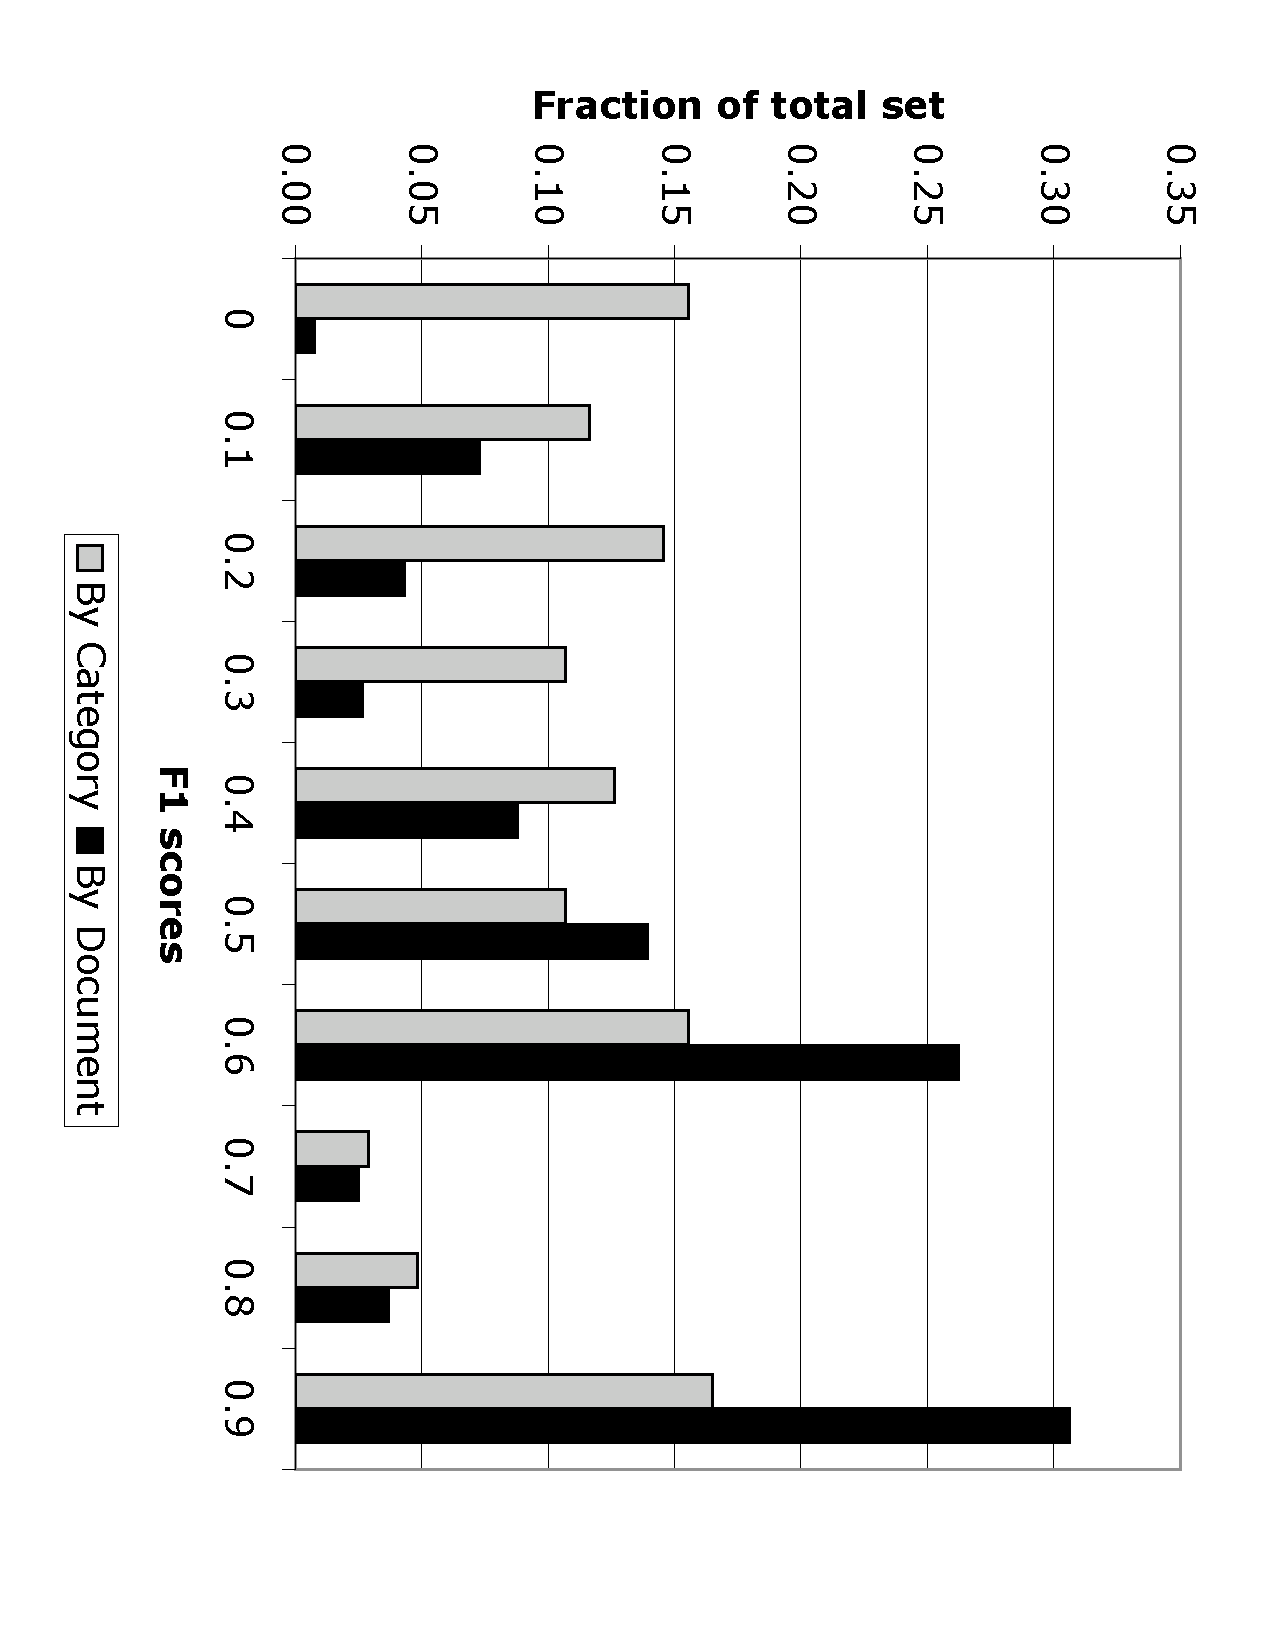
\includegraphics[width=5cm]{results.epsf}
\caption{Histogram of report type results for different performance ranges}
\label{histogram}
\end{figure}

\section{Conclusions}

In this paper we have applied several machine learning techniques (Neural Networks, Na�ve Bayes, and Support Vector Machines) to the categorization of announcements of companies publicly traded by the ASX.  Two tasks were evaluated: the categorization of documents as sensitive or not, and the categorization in one of the 144 report types defined by ASX. The results show that is possible to obtain classifiers with more than 88\% precision and recall on the sensitivity task and 86\% precision, 74\% recall on the report type task.

The results are somewhat better than the ones obtained by several researchers working on the Reuters news cable database \cite{calvo:00} \cite{calvo:01}. This database has fewer categories (90) than the report type task but also fewer documents (10,000). Although it is risky to try to extrapolate the results, we believe that due to the similarity in the documents, other financial databases with documents in English should also have similar performance. Future work includes testing adding statistical feature selection to the classification framework, and improving the efficiency of the algorithms so they can be used for even larger data sets. 

The excellent performance shows the possibility to use these classifiers in commercial applications for both tasks, sensitivity detection and report type categorization.

\section{Acknowledgements}

The authors gratefully acknowledge financial support from the Capital Markets Collaborative Research Centre and the University of Sydney.

\section{References}

...


\bibliographystyle{plain}
\bibliography{/Users/ken/src/tcframe/ref/TC-references}

\end{document}
